\section{Introducción}
			
\begin{frame}{Grafeno}
	\justifying
	\begin{multicols}{2}

		\underline{Grafeno}:\\ 
		Es una de las formas alotrópicas del carbono, entre las que se encuentran el grafito, diamante, entre otras. En la cual los átomos están organizados en un arrreglo bidimensional y con un patrón hexagonal en forma de panel de abeja.

		\begin{figure}
		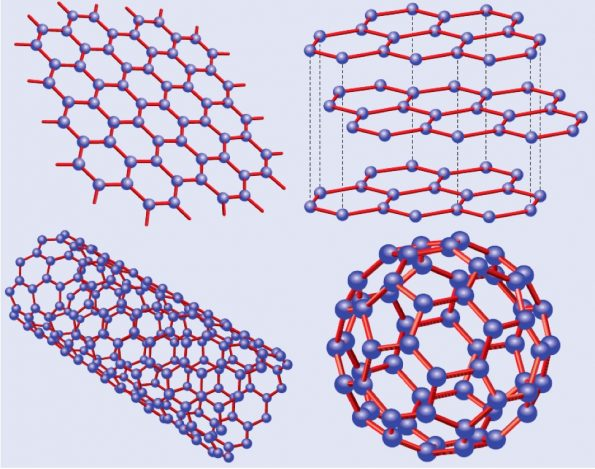
\includegraphics[width=5.5cm]{graficas/alotropo.jpg}
		\caption{ Alótropos del carbono. \textit{Tomado de }\cite{Neto2006}} 
		\label{grafeno}
		\end{figure}
	\end{multicols}
\end{frame}

\begin{frame}
	\begin{multicols}{2}
		Los electrones en el grafeno se comportan como fermiones de Dirac sin masa \cite{Katsnelson2007}. A temperatura ambiente, los electrones pueden viajar varias micras sin presentar dispersión. Es buen conductor, resistente y transparente.
		\begin{figure}
			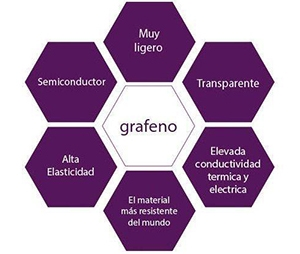
\includegraphics[width=5.5cm]{graficas/propiedadesGrafeno.jpg}
			\caption{Propiedades del grafeno}
		\end{figure}
		\end{multicols}
\end{frame}

\begin{frame}
	Las oscilaciones magnéticas son un fenómeno bien conocido en la física de la materia condensada, aunque se necesitan temperaturas muy bajas para observarlos. En el grafeno, persiste incluso a temperaturas ambiente. Ésto se atribuye a la periodicidad de las superredes de grafeno\cite{Kumar2017}.

	\begin{figure}
		\subfigure[Superred de grafeno]{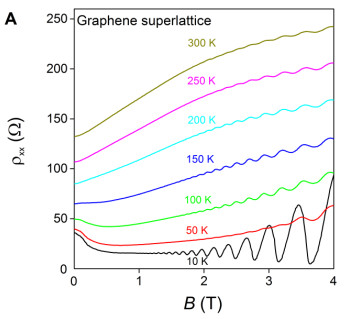
\includegraphics[width=4cm]{graficas/oscilaciones_superred.jpg}}
		\subfigure[grafeno]{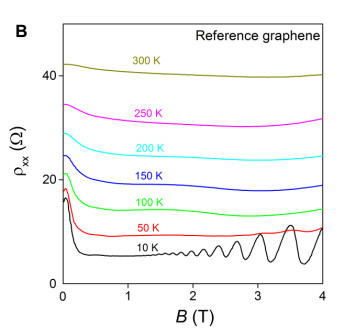
\includegraphics[width=4cm]{graficas/oscilaciones_grafeno.jpg}}
	\caption{$\rho$ vs $B$ a diferentes temperaturas. \textit{Tomadas de \cite{Kumar2017}}}
	\end{figure}
\end{frame}

\begin{frame}
	\begin{multicols}{2}
		Las oscilaciones cuánticas involucran trayectorias ciclotrónicas y pueden originarse debido a la geometría de la muestra \cite{Chen2014}. Lo que conlleva a la cuantización de Landau(L.L.) y a oscilaciones de Shubnikov-de Hass (SdH) \cite{Fujita2014}.
		Incluso en el grafeno, las oscilaciones SdH raramente persisten a temperaturas superiores a los 100K \cite{Kishigi2014}, se necesitan campos magnéticos grandes para observarlas \cite{Novoselov2007}
	\end{multicols}
\end{frame}

\begin{frame}
	\begin{multicols}{2}
		Los sistemas electrónicos tambien presentan oscilaciones magnéticas. Los espectros autosimilares son referidos a las mariposas de Hofstadter (HB) \cite{Yu2014}-\cite{Yang2016}.\\
		Se han reportado estudios de transporte eléctrico en superredes de grafeno colocado sobre una base de nitruro de boro hexagonal (h-BN) \cite{Yankowitz2012}, lo que permite que se observe las características de las HB originadas en la superred en un campo magnético de algunos Teslas (T) \cite{BenShalom2016}
		\begin{figure}
			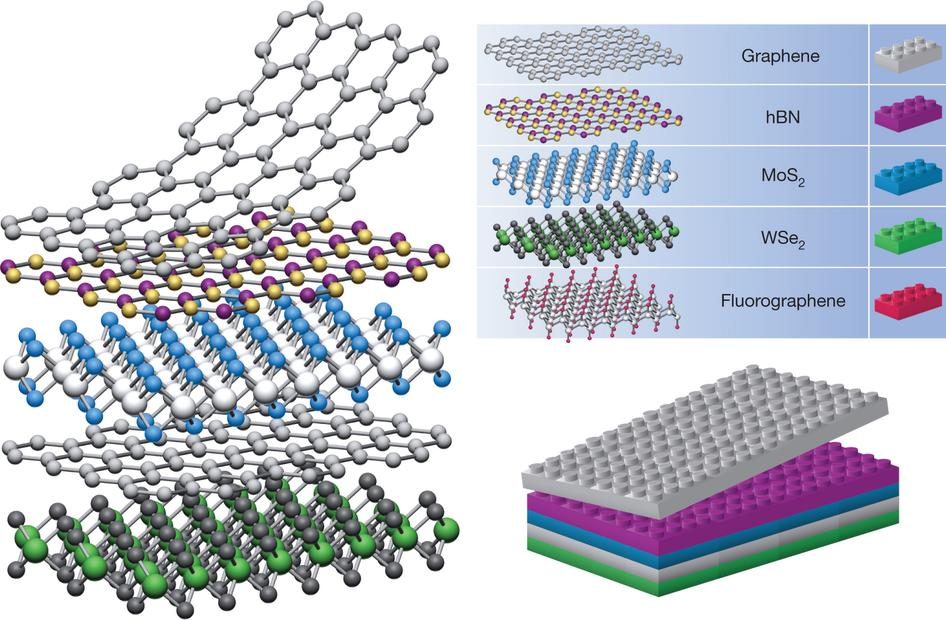
\includegraphics[width=6cm]{graficas/heterostructures.jpg}
			\caption{Superredes de grafeno. \textit{Tomado de} \cite{Geim2013}}
			\label{heterostructures}
		\end{figure}
	\end{multicols}
\end{frame}

\begin{frame}
	El estudio de estas oscilaciones magnéticas ha adquirido un gran impulso debido a las recientes observaciones experimentales de las oscilaciones magnéticas a altas temperaturas en sistemas basados en grafeno debido a la emergente periodicidad de estados de Bloch delocalizados en campos magnéticos altos, llamadas oscilaciones de Brown-Zak (BZ). \\
	

	En este contexto, el presente trabajo pretende ahondar en el estudio de las propiedades magneto-oscilatorias de las estructuras basadas en grafeno en presencia de un campo magnético a altas temperaturas.

\end{frame}
